% chktex-file 2% chktex-file 29
% chktex-file 13
\documentclass{report}
\usepackage{setspace}
\usepackage[a4paper, total={7in, 10in}]{geometry}
\usepackage[fleqn]{amsmath}
\usepackage{empheq}
\usepackage{amssymb}
\usepackage{amsthm}
\usepackage{gensymb}
\usepackage[fleqn]{cases}
\usepackage{multicol}
\usepackage{color}
\usepackage{stix}
\usepackage{chngcntr}
\usepackage{tikz}
\usepackage{enumitem}
\usepackage{pgfplots}
\usepackage{etoolbox}
\usepackage{tikz-3dplot}
\usepackage{tkz-euclide}
\usepackage{enumitem}

\def\nswe#1#2#3{#1\,$#2^\circ\,#3'$}
\graphicspath{ {./assets/} }
\usetikzlibrary{calc,matrix,arrows}
\usetikzlibrary{decorations.pathmorphing,patterns, calligraphy, perspective,backgrounds}

\counterwithout{equation}{chapter}
\setlength{\columnseprule}{1pt}
\setlength{\columnsep}{24pt}
\setcounter{chapter}{16}
\hfuzz=100pt

\newcommand{\pgfplotsdrawaxis}{\pgfplots@draw@axis}
\makeatother
\pgfplotsset{only axis on top/.style={axis on top=false, after end axis/.code={
                    \pgfplotsset{axis line style=opaque, ticklabel style=opaque, tick style={thick,opaque},
                        grid=none}\pgfplotsdrawaxis}}}

\newtheorem{theorem}{Theorem}

\begin{document}

\makeatletter
\newcommand{\newparallel}{\mathrel{\mathpalette\new@parallel\relax}}
\newcommand{\new@parallel}[2]{%
    \begingroup
    \sbox\z@{$#1T$}% get the height of an uppercase letter
    \resizebox{!}{\ht\z@}{\raisebox{\depth}{$\m@th#1/\mkern-5mu/$}}%
    \endgroup
}
\makeatother

\newcommand{\sol}[1]{

    \noindent \textbf{Sol.}
}
\newcommand{\prooff}[1]{

    \noindent \textbf{Proof.}
}
\newcommand\m[1]{\begin{pmatrix}#1\end{pmatrix}}
\newcommand\vm[1]{\begin{vmatrix}#1\end{vmatrix}}
\newenvironment{amatrix}[1]{%
    \left(\begin{array}{@{}*{#1}{c}|c@{}}
        }{%
    \end{array}\right)
}
\newenvironment{cequation}{
    \makeatletter
    \setbool{@fleqn}{false}
    \makeatother
    \begin{equation*}
        }{\end{equation*}}

\begin{titlepage}
    \raggedleft{}
    \rule{1pt}{\textheight}
    \hspace{0.02\textwidth}
    \parbox[b]{0.75\textwidth}{

    {\Huge\bfseries Solution Book of \\[0.5\baselineskip] Mathematic}\\[2\baselineskip]
    {\large\textit{Ssnior 2 Part I}}\\[4\baselineskip]
    {\Large\textsc{MELVIN CHIA}}

    \vspace{0.5\textheight}

    {\noindent Written on 9 October 2022}\\[\baselineskip]
    }

\end{titlepage}

\doublespacing{}
\tableofcontents
\singlespacing{}
\newpage

\begin{multicols}{2}
    \begin{enumerate}
        \item The diagram below shows a right pyramid with lateral edges of $18cm$, its base
              $ABCD$ is a rectangle with length of $15cm$ and width of $10cm$. Find:
              \begin{enumerate}
                  \item The height of the pyramid.
                  \item The angle formed by plane $VAB$ and plane $ABCD$.
                  \item The angle formed by plane $VBC$ and plane $VAD$.
              \end{enumerate}
              \begin{center}
                  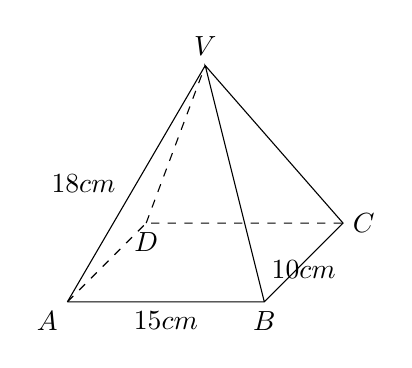
\begin{tikzpicture}
                      \tikzstyle{point}=[circle,thick,draw=black,fill=black,inner sep=0pt,minimum width=4pt,minimum height=4pt]
                      \node (a) at (0,0) {};
                      \node (b) at (2.5,0) {};
                      \node (c) at (3.5,1) {};
                      \node (d) at (1,1) {};
                      \node (e) at (1.75,3) {};
                      \draw (a.center) node [below left] {$A$} -- (b.center) node [below] {$B$} node [midway, below] {$15cm$} -- (c.center) node [ right] {$C$} node [midway, right=12pt, below=-4pt] {$10cm$} -- (e.center) node [above] {$V$} -- (b.center);
                      \draw (a.center) -- (e.center) node [midway, left=4pt] {$18cm$};
                      \draw[dashed] (a.center) -- (d.center) -- (c.center);
                      \draw[dashed] (d.center) node [below] {$D$} -- (e.center);
                  \end{tikzpicture}
              \end{center}
        \item The diagram below shows a right prism with isoceles triangle bases. The side
              length and base length of the triangle base are $10cm$ and $16cm$ respectively,
              the height of the prism is $20cm$. Given that $P$ is the midpoint of $AB$.
              Find:
              \begin{enumerate}
                  \item The length of $PC$.
                  \item The angle formed by line $EC$ and plane $ABCD$.
                  \item The angle formed by plane $DCE$ and plane $ABCD$.
              \end{enumerate}
              \begin{center}
                  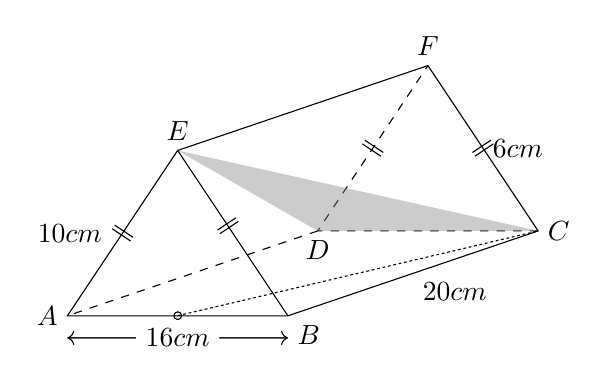
\begin{tikzpicture}[scale=1.4]
                      \draw (1,1.5,2) node [above] {$E$} --(2.5,1.5,0) --(3.5,0,0) node [right] {$C$} node [midway, right] {$6cm$} --(2,0,2) node [below right] {$B$}  node [midway, below right] {$20cm$} --(0,0,2) node [left] {$A$}  --(1,1.5,2) node [midway, left=4pt] {$10cm$};
                      \draw (1,1.5,2)--(2,0,2);
                      \draw[dashed](3.5,0,0)--(1.5,0,0) node [below] {$D$}--(2.5,1.5,0) node [above] {$F$};
                      \draw[dashed](1.5,0,0)--(0,0,2);
                      \fill[color=gray, opacity=0.4] (1, 1.5, 2) -- (3.5, 0, 0) -- (1.5, 0, 0);
                      \draw (0, -1, -0.6) circle (1pt);
                      \draw [dash pattern=on 1pt off 1pt] (0, -1, -0.6) -- (3.5, 0, 0);
                      \path (0, -0.2, 2) -- node (success) {$16cm$} (2, -0.2, 2);
                      \draw[->] (0, -0.2, 2) -- (success) -- (2, -0.2, 2);
                      \draw[->] (2, -0.2, 2) -- (success) -- (0, -0.2, 2);
                      \node (a) at (1,1.5,2) {};
                      \node (b) at (2, 0, 2) {};
                      \node (c) at (0,0,2) {};
                      \node (d) at (1.5, 0, 0) {};
                      \node (e) at (2.5, 1.5, 0) {};
                      \node (f) at (3.5, 0, 0) {};
                      \tkzMarkSegment[pos=.45,mark=||](a,b);
                      \tkzMarkSegment[pos=.5,mark=||](a,c);
                      \tkzMarkSegment[pos=0.5,mark=||](e,f);
                      \tkzMarkSegment[pos=0.5,mark=||](e,d);
                  \end{tikzpicture}
              \end{center}
    \end{enumerate}
\end{multicols}
\end{document}